\documentclass[10pt,a4paper]{article}
\usepackage[utf8]{inputenc}
\usepackage{amsmath}
\usepackage{amsfonts}
\usepackage{amssymb}
\usepackage{hyperref}

\usepackage[usenames,dvipsnames]{xcolor}
\usepackage{tikz}

\usetikzlibrary{arrows,shapes,automata,positioning,calc}

\usepackage{caption}
\usepackage{subcaption}

\hypersetup{
    colorlinks=true,
    linkcolor=blue,
    filecolor=magenta,      
    urlcolor=cyan,
    pdftitle={Overleaf Example},
    pdfpagemode=FullScreen,
    }

\usepackage{amsmath}
\DeclareMathOperator*{\argmax}{arg\,max}

\title{Chapter 3 - Finite Markov Decision Processes}
\author{Stéphane Liem NGUYEN}
\begin{document}
\maketitle

Exercises with (\textbf{\textit{corrected}}) were corrected based on the \href{http://incompleteideas.net/book/errata.html}{Errata}

These are my own answers and mistakes or errors are possible.

\paragraph{\textit{Exercise 3.1} (p. 51)} Devise three example tasks of your own that fit into the MDP framework, identifying for each its states, actions, and rewards. Make the three examples as \textit{different} from each other as possible. The framework is abstract and flexible and can be applied in
many different ways. Stretch its limits in some way in at least one of your examples.

\paragraph{\textit{Exercise 3.2} (p. 51)} Is the MDP framework adequate to usefully represent \textit{all} goal-directed learning tasks? Can you think of any clear exceptions ?

\paragraph{\textit{Exercise 3.3} (p. 51)} Consider the problem of driving. You could define the actions in terms of the accelerator, steering wheel, and brake, that is, where your body meets the machine.
Or you could define them farther out---say, where the rubber meets the road, considering your actions to be tire torques.
Or you could define them farther in---say, where your brain meets your body, the actions being muscle twitches to control your limbs.
Or you could go to a really high level and say that your actions are your choices of \textit{where} to drive.
What is the right level, the right place to draw the line between agent and environment?
On what basis is one location of the line to be preferred over another? Is there any
fundamental reason for preferring one location over another, or is it a free choice?

\paragraph{\textit{Exercise 3.4} (p. 53)} Give a table analogous to that in Example $3.3$ (recycling robot), but for $p(s', r \lvert s, a)$. It should have columns for $s, a, s', r$, and $p(s', r|s, a)$, and a row for every $4$-tuple for which $p(s', r \lvert s, a) > 0$.

\paragraph{\textit{Exercise 3.5} (p. 55)} The equations in Section $3.1$ (Agent-Environment Interface) are for the continuing case and need to be modified (very slightly) to apply to episodic tasks. Show that you know the modifications needed by giving the modified version of ($3.3$).

\bigskip
Based on the book at page $54$: "Episodes can all be considered to
end in the same terminal state, with different rewards for the different outcomes. [...] In episodic tasks we sometimes need
to distinguish the set of all nonterminal states, denoted $\mathcal{S}$, from the set of all states plus the terminal state, denoted $\mathcal{S}^+$.", we can just add the terminal state to set of possible next states.

We can rewrite the modified version of ($3.3$) as follows:

\begin{equation}
\sum_{s' \in \mathcal{S}^{\color{red}+\color{black}}} \sum_{r \in \mathcal{R}} p(s', r | s, a) = 1,\quad \forall s \in \mathcal{S}, \forall a \in \mathcal{A}(s)
\end{equation}

where $s'$ can be the terminal state.



\paragraph{\textit{Exercise 3.6} (p. 56)} Suppose you treated pole-balancing as an episodic task but also used discounting, with all rewards zero except for $-1$ upon failure. What then would the return be at each time? How does this return differ from that in the discounted, continuing formulation of this task?

\bigskip
The return for the discounted, \textit{episodic} formulation would be at each time
\begin{equation}
\begin{split}
G_t &\doteq R_{t+1} + \gamma R_{t+2} + \gamma^2 R_{t+3} + \hdots + \gamma^{T-1} R_T\\
&= -\gamma^{T-1}
\end{split}
\end{equation}
while the return for the discounted, \textit{continuing} formulation would be at each time
\begin{equation}
\begin{split}
G_t &\doteq \sum_{k=0}^\infty \gamma^k R_{t+k+1} = - \sum_{k=0}^\infty \gamma^k \textbf{1}_{\textrm{failure}}
\end{split}
\end{equation}

\paragraph{\textit{Exercise 3.7} (p. 56)} Imagine that you are designing a robot to run a maze. You decide to give it a reward of $+1$ for escaping from the maze and a reward of zero at all other times. The task seems to break down naturally into episodes---the successive runs through the maze---so
you decide to treat it as an episodic task, where the goal is to maximize expected total reward ($3.7$). After running the learning agent for a while, you find that it is showing no improvement in escaping from the maze. What is going wrong? Have you effectively communicated to the agent what you want it to achieve?

\bigskip
We can just recall that the return $G_t$ from ($3.7$) (for episodic tasks) is just the sum of the future rewards.
\begin{equation}
G_t \doteq R_{t+1} + R_{t+2} + R_{t+3} + \hdots + R_T
\end{equation}

Because of how we defined the rewards and because we use the undiscounted formulation of the return, $G_t$ is either $1$ or $0$ (if a game can terminate without escape from the maze) and what we try to maximize is the expected amount of games where we escape from the maze. For a given state, its value (not estimation) would be the average amount of future games where we will escape if we follow some policy.

%If we suppose that the exit is reachable from any state, then the values of all states (not estimations) could be the same at each time step.
\textbf{Work In Progress}

\paragraph{\textit{Exercise 3.8} (p. 56)} Suppose $\gamma = 0.5$ and the following sequence of rewards is received $R_1 = -1,
R_2 = 2, R_3 = 6, R_4 = 3$, and $R_5 = 2$, with $T = 5$. What are $G_0, G_1, \hdots, G_5$? Hint:
Work backwards.

\bigskip
\begin{itemize}
\item $G_5=0$
\item $G_4=R_5 + \gamma \cdot G_5 = 2 + 0.5 \cdot 0 = 2$
\item $G_3=R_4 + \gamma \cdot G_4 = 3 + 0.5 \cdot 2 = 4$
\item $G_2=R_3 + \gamma \cdot G_3 = 6 + 0.5 \cdot 4 = 8$
\item $G_1=R_2 + \gamma \cdot G_2 = 2 + 0.5 \cdot 8 = 6$
\item $G_0=R_1 + \gamma \cdot G_1 = -1 + 0.5 \cdot 6 = 2$
\end{itemize}

\paragraph{\textit{Exercise 3.9} (p. 56)} Suppose $\gamma = 0.9$ and the reward sequence is $R_1 = 2$ followed by an infinite sequence of $7$s. What are $G_1$ and $G_0$?

\bigskip
Instead of having an episodic task as the previous exercise, we use the discounted, continuing formulation of the return
\begin{equation}
G_t \doteq \sum_{k=0}^\infty \gamma^k R_{t+k+1}
\end{equation}

$G_1$ is directly given by
\begin{equation}
G_1 \doteq \sum_{k=0}^\infty \gamma^k R_{k+2} = 7 \sum_{k=0}^\infty \gamma^k = 7 \cdot \frac{1}{1-\gamma} = 70
\end{equation}

by using ($3.10$) from the book.

Finally, $G_0 = R_1 + \gamma \cdot G_1 = 2 + 0.9 \cdot 70 = 65$.


\paragraph{\textit{Exercise 3.10} (p. 56)} Prove the second equality in ($3.10$).

\bigskip
We want to prove that in the continuing tasks, if the rewards at all time steps are constant $+1$, then the return is $\frac{1}{1-\gamma} < \infty$ for $0 \leq \gamma < 1$
\begin{equation}
G_t =\sum_{k=0}^\infty \gamma^k = \frac{1}{1-\gamma}
\end{equation}

We first pass the $1-\gamma$ on the other side and do some manipulations to complete the proof
\begin{equation}
(1-\gamma) \sum_{k=0}^\infty \gamma^k = 1 \iff \sum_{k=0}^\infty \gamma^k - \sum_{k=1}^\infty \gamma^{k} = \gamma^0 + 0 = 1
\end{equation}

\paragraph{\textit{Exercise 3.11} (p. 58)} If the current state is $S_t$, and actions are selected according to a stochastic
policy $\pi$, then what is the expectation of $R_{t+1}$ in terms of $\pi$ and the four-argument dynamics function $p$ ($3.2$)?

\bigskip
\begin{equation}
\mathbb{E}_\pi[R_{t+1} \lvert S_t=s] = \sum_{a} \pi(a \lvert s) \sum_{s', r} p(s', r \lvert s, a) r
\end{equation}
where $a \in \mathcal{A}(s), r \in \mathcal{R}$, $s$ and $s' \in \mathcal{S}$.

Remark: We can also rewrite (not asked in the exercise) the equality as follows:
\begin{equation}
\mathbb{E}_\pi[R_{t+1} \lvert S_t=s] = \sum_{a} \pi(a \lvert s) r(s, a)
\end{equation}

\paragraph{\textit{Exercise 3.12} (p. 58)} Give an equation for $v_\pi$ in terms of $q_\pi$ and $\pi$.

\bigskip
\begin{equation}
\begin{split}
v_\pi(s) &= \sum_{a} \pi(a \lvert s) \mathbb{E}_\pi[G_t \lvert S_t = s, A_t = a]\\
&= \sum_{a} \pi(a \lvert s) q_\pi(s, a)
\end{split}
\end{equation}

\paragraph{\textit{Exercise 3.13} (p. 58)} Give an equation for $q_\pi$ in terms of $v_\pi$ and the four-argument $p$.

\bigskip
\begin{equation}
q_\pi(s, a) = \sum_{s', r} p(s', r \lvert s, a) \left[r + \gamma v_\pi(s') \right]
\end{equation}

\paragraph{\textit{Exercise 3.14} (p. 60)} The Bellman equation ($3.14$) must hold for each state for the value function $v_\pi$ shown in Figure $3.2$ (right) of Example $3.5$ (Gridworld). Show numerically that this equation holds for the center state, valued at $+0.7$, with respect to its four neighboring states, valued at
$+2.3, +0.4, -0.4$, and $+0.7$. (These numbers are accurate only to one decimal place.)

\bigskip
Let's recall the Bellman expectation equation for the state-value function $v_\pi$
\begin{equation}
v_\pi(s) = \sum_{a} \pi(a \lvert s) \sum_{s', r} p(s', r \lvert s, a) \left[r + \gamma v_\pi(s')\right]
\end{equation}

and that the example used a discount rate/factor $\gamma$ of $0.9$. We also have to recall that the policy $\pi$ is an equiprobable random one and that the agent transitions deterministically to a future state and get deterministically a reward of $0$, $-1$, $10$ or $5$.

We can now show numerically that the equation holds for the center state:
\begin{equation}
\begin{split}
0.25 \cdot [0.9 \cdot 2.3] + 0.25 \cdot [0.9 \cdot 0.4] + 0.25 \cdot [0.9 \cdot -0.4] + 0.25 \cdot [0.9 \cdot 0.7] &= 9/40 \cdot 3\\
&= 0.675\\
&\approx 0.7
\end{split}
\end{equation}
because all the immediate rewards were $0$.

\paragraph{\textit{Exercise 3.15} (p. 61)} In the gridworld example, rewards are positive for goals, negative for running into the edge of the world, and zero the rest of the time. Are the signs of these rewards important, or only the intervals between them? Prove, using ($3.8$), that adding a
constant $c$ to all the rewards adds a constant, $v_c$, to the values of all states, and thus does not affect the relative values of any states under any policies. What is $v_c$ in terms of $c$ and $\gamma$?

\bigskip
We can first note that the gridworld example is a continuing task. For continuing tasks, we will show that shifting all rewards by a constant $c$ leaves the task unchanged and consequently, only the intervals between rewards are important. Signs of the rewards can change by shifting the rewards.

\bigskip
Let's denote $\hat{G}_t$ the new return after shifting all the rewards by $c$ and $G_t$ the return before shifting. We can show the relation between $G_t$ and $\hat{G}_t$
\begin{equation}\label{eq_continuing_shift_return}
\hat{G}_t \doteq \sum_{k=0}^\infty \gamma^k (c + R_{t+k+1}) = G_t + \frac{c}{1-\gamma} = G_t + v_c
\end{equation}
where $v_c = \frac{c}{1-\gamma}$ and the second equality comes from the definition of the return for the discounted continuing case and from the ($3.10$) of the book. 

As direct consequence of the equation \ref{eq_continuing_shift_return}, the values of all states $\hat{v}_\pi$ after shifting the rewards by $c$ can be written as:
\begin{equation}
\begin{split}
\hat{v}_\pi(s) &\doteq \mathbb{E}_\pi[\hat{G}_t \lvert S_t = s]\\
&= \mathbb{E}_\pi[ G_t + v_c \lvert S_t = s] = v_\pi(s) + v_c
\end{split}
\end{equation}
because $v_c$ is a constant and $G_t$ is a random variable.

We can then conclude that the goal of the agent is left unchanged, the maximization of expected total reward will lead to the same goal.

\paragraph{\textit{Exercise 3.16} (p. 61)} Now consider adding a constant $c$ to all the rewards in an episodic task, such as maze running. Would this have any effect, or would it leave the task unchanged as in the continuing task above? Why or why not? Give an example.

\bigskip
If we add a constant $c$ to all the rewards in an episodic task, the task will change because the new return depends on the final time step $T$. If we take the same notations as the previous exercise, we get
\begin{equation}\label{eq_episodic_shift_return}
\hat{G}_t \doteq \sum_{k=t+1}^T (c + R_k) = G_t + c \cdot (T - t) = G_t + f_c(T)
\end{equation}
where now the new return depends on a function of $T$; $f_c(T) = c \cdot (T - t)$ that is not anymore a constant.

As effect on the state values, we have that
\begin{equation}\label{eq_episodic_shift_return_state_values}
\begin{split}
\hat{v}_\pi(s) &\doteq \mathbb{E}_\pi[\hat{G}_t \lvert S_t = s]\\
&= \mathbb{E}_\pi[ G_t + c \cdot (T - t) \lvert S_t = s] = v_\pi(s) + c \cdot \mathbb{E}_\pi[(T - t) \lvert S_t = s]
\end{split}
\end{equation}

where $c \cdot \mathbb{E}_\pi[T - t \lvert S_t = s]$ can be positive or negative (depending on the value of $c$). By adding that constant $c$, maximizing the new expected total reward is different from maximizing the old expected total reward.

As example in maze running, if we suppose that $R_k = -1$ at each time step $k$ and $c = 1$ then the new values of all states would be $0$ based on equation \ref{eq_episodic_shift_return} and the goal would not even exist anymore. The old state value function is cancelled by the expected number of time steps left in equation \ref{eq_episodic_shift_return_state_values}.


\clearpage
\paragraph{\textit{Exercise 3.17} (p. 61)} What is the Bellman equation for action values, that is, for $q_\pi$? It must give the action value $q_\pi(s, a)$ in terms of the action values, $q_\pi(s', a')$, of possible successors to the state–action pair ($s, a$).
Hint: The backup diagram in Figure  \ref{bellman_eq_action_val} corresponds to this equation.
Show the sequence of equations analogous to ($3.14$), but for action
values.


\begin{figure}[h]
\centering
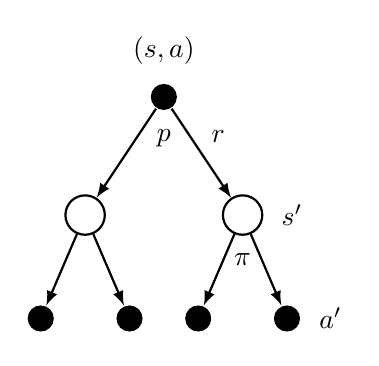
\begin{tikzpicture}[
>=latex, thick ,bend angle=8,auto,
state-node/.style = {circle,thick,draw=black,minimum size=5mm},
action-node/.style = {circle,fill=black, radius=2.5mm, minimum size=2.5mm}
]
   
\node [action-node] (root) at (0, 0) {};
\node [state-node] (l) at (-1, -1.5) {};
\node [state-node] (r) at (1, -1.5) {};
\node [action-node, below left=1cm and 0.25cm of l] (ll) {};
\node [action-node, below right=1cm and 0.25cm of l] (lr) {};
\node [action-node, below left=1cm and 0.25cm of r] (rl) {};
\node [action-node, below right=1cm and 0.25cm of r] (rr) {};

% labels
\node [above=1mm of root] {$(s, a)$};
\node [below=1mm of root] {$p$};
\node [right=1mm of r] {$s'$};
\node [below=1mm of r] {$\pi$};
\node [right=1mm of rr] {$a'$};

% arrows
\draw[->] (root) -- (l);
\draw[->] (root) -- node[midway]{$r$} (r);
\draw[->] (l) -- (ll);
\draw[->] (l) -- (lr);
\draw[->] (r) -- (rl);
\draw[->] (r) -- (rr);


\end{tikzpicture}
\caption{$q_\pi$ backup diagram}
\label{bellman_eq_action_val}
\end{figure}

\begin{equation}
\begin{split}
q_\pi(s, a) &\doteq \mathbb{E}_\pi[G_t \lvert S_t = s, A_t = a]\\
&= \mathbb{E}_\pi[R_{t+1} + \gamma G_{t+1}\lvert S_t = s, A_t = a]\\
&= \sum_{s', r} p(s', r \lvert s, a) \left[r + \gamma \sum_{a'} \pi(a' \lvert s') \mathbb{E}_\pi[G_{t+1} \lvert S_{t+1} = s', A_{t+1} = a']\right]\\
&= \sum_{s', r} p(s', r \lvert s, a) \left[r + \gamma \sum_{a'} \pi(a' \lvert s') q_\pi(s', a')\right]
\end{split}
\end{equation}

\paragraph{\textit{Exercise 3.18} (p. 62)} The value of a state depends on the values of the actions possible in that state and on how likely each action is to be taken under the current policy. We can
think of this in terms of a small backup diagram rooted at the state and considering each
possible action:

\begin{figure}[h]
\centering
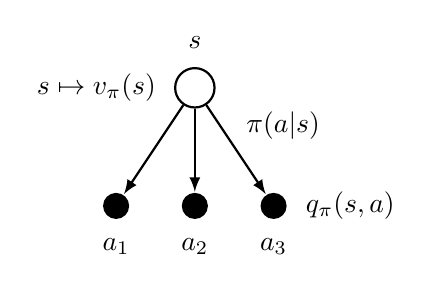
\begin{tikzpicture}[
>=latex, thick ,bend angle=8,auto,
state-node/.style = {circle,thick,draw=black,minimum size=5mm},
action-node/.style = {circle,fill=black, radius=2.5mm, minimum size=2.5mm}
]
   
\node [state-node] (root) at (0, 0) {};
\node [action-node] (l) at (-1, -1.5) {};
\node [action-node] (m) at (0, -1.5) {};
\node [action-node] (r) at (1, -1.5) {};


% labels
\node [above=1mm of root] {$s$};
\node [left=1mm of root] {$s \mapsto v_\pi(s)$};
\node [right=1mm of r] {$q_\pi(s, a)$};
\node [below=1mm of l] {$a_1$};
\node [below=1mm of m] {$a_2$};
\node [below=1mm of r] {$a_3$};


% arrows
\draw[->] (root) -- (l);
\draw[->] (root) -- (m);
\draw[->] (root) -- node[midway]{$\pi(a | s)$} (r);


\end{tikzpicture}
\caption{Small backup diagram showing $v_\pi$ in terms of $q_\pi$ and the policy $\pi$}
\label{relation_state_value_action_value}
\end{figure}


Give the equation corresponding to this intuition and diagram for the value at the root node, $v_\pi(s)$, in terms of the value at the expected leaf node, $q_\pi(s, a)$, given $S_t = s$. This equation should include an expectation conditioned on following the policy, $\pi$. Then give
a second equation in which the expected value is written out explicitly in terms of $\pi(a|s)$ such that no expected value notation appears in the equation.

\bigskip
\begin{equation}
\begin{split}
v_\pi(s) &\doteq \mathbb{E}_\pi[G_t \lvert S_t = s] = \mathbb{E}_\pi\left[\mathbb{E}_\pi[G_t \lvert S_t, A_t] \lvert S_t = s\right]\\
&= \mathbb{E}_\pi[q_\pi(S_t, A_t) \lvert S_t = s]\\
&= \sum_{a} \pi(a \lvert s) q_\pi(s, a)
\end{split}
\end{equation}

by using the Law of iterated expectations.

\paragraph{\textit{Exercise 3.19} (p. 62)} The value of an action, $q_\pi(s, a)$, depends on the expected next reward and
the expected sum of the remaining rewards. Again we can think of this in terms of a
small backup diagram, this one rooted at an action (state-action pair) and branching to
the possible next states:

\begin{figure}[h]
\centering
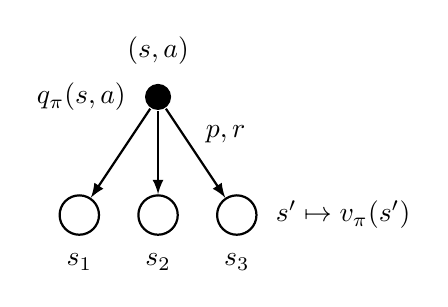
\begin{tikzpicture}[
>=latex, thick ,bend angle=8,auto,
state-node/.style = {circle,thick,draw=black,minimum size=5mm},
action-node/.style = {circle,fill=black, radius=2.5mm, minimum size=2.5mm}
]
   
\node [action-node] (root) at (0, 0) {};
\node [state-node] (l) at (-1, -1.5) {};
\node [state-node] (m) at (0, -1.5) {};
\node [state-node] (r) at (1, -1.5) {};

% labels
\node [above=1mm of root] {$(s, a)$};
\node [left=1mm of root] {$q_\pi(s, a)$};
\node [right=1mm of r] {$s' \mapsto v_\pi(s')$};
\node [below=1mm of l] {$s_1$};
\node [below=1mm of m] {$s_2$};
\node [below=1mm of r] {$s_3$};

% arrows
\draw[->] (root) -- (l);
\draw[->] (root) -- (m);
\draw[->] (root) -- node[midway]{$p, r$} (r);


\end{tikzpicture}
\caption{Small backup diagram showing $q_\pi$ in terms of $v_\pi$ and the dynamics function $p$}
\label{relation_action_value_state_value}
\end{figure}


Give the equation corresponding to this intuition and diagram for the action value, $q_\pi(s, a)$, in terms of the expected next reward, $R_{t+1}$, and the expected next state value, $v_\pi(S_{t+1})$, given that $S_t=s$ and $A_t=a$. This equation should include an expectation but
\textit{not} one conditioned on following the policy.
Then give a second equation, writing out the expected value explicitly in terms of $p(s', r \lvert s, a)$ defined by ($3.2$), such that no expected value notation appears in the equation.

\bigskip
\begin{equation}
\begin{split}
q_\pi(s, a) &\doteq \mathbb{E}_\pi[G_t \lvert S_t = s, A_t = a] \\
&= \mathbb{E}_\pi[R_{t+1} + \gamma G_{t+1} \lvert S_t = s, A_t = a]]\\
&= \mathbb{E}[R_{t+1} + \gamma v_\pi(S_{t+1}) \lvert S_t = s, A_t = a]]\\
&= \sum_{s', r} p(s', r \lvert s, a) \left[r + \gamma v_\pi(s') \right]
\end{split}
\end{equation}


\paragraph{\textit{Exercise 3.20} (p. 66)} 
Draw or describe the optimal state-value function for the golf example.

\bigskip
The optimal state-value function for the golf example tells us the negative of
the number of strokes to the hole from a given state if actions are selected optimally.

%Let's first determine the regions for the optimal state-value before their values.

By using the information from the Figure $3.3$ in the book, we know that the first stroke with the driver will move the ball in the $-2$ region from the contour plot of $q_*(s, \textrm{\textbf{driver}})$ while the putter only moves to the $-5$ region for the upper part of the figure. We must only keep in the mind the difference of the values between neighbouring regions from the upper part of the figure because the values of the states are not based on the optimal policy. Based on "Intuitively, the Bellman optimality equation expresses the
fact that the value of a state under an optimal policy must equal the expected return for
the best action from that state" from page $63$ and the previous remarks, the first region is the same (as well as its value) as for the contour plot of $q_*(s, \textrm{\textbf{driver}})$ (the optimal first action from the tee is by using the driver).

The first region has then a value of $-3$ indicating that the optimal strategy is to perform $3$ actions from the tee to the hole. By comparing again the contour plot of both value functions, it is not optimal to use the putter from the $-2$ region of the lower graph because even if the best we can obtain from that region is if the first action with the driver from the tee threw the ball in the green area, the first action with the driver has the risk of throwing the ball in the sand traps. If the ball falls in the sand traps, the putter is useless to get the ball out of them. The second optimal action is then to use again the driver and the region we keep for the optimal state-value function is the same as for the optimal action-value function $q_*(s, \textrm{\textbf{driver}})$ with value $-2$.

The last region is again the same.

\textbf{Work In Progress}

\paragraph{\textit{Exercise 3.21} (p. 66)} 
Draw or describe the contours of the optimal action-value function for
putting, $q_*(s, \textrm{\textbf{putter}})$, for the golf example.

\bigskip
The optimal action-value function for putting, $q_*(s, \textrm{\textbf{putter}})$, shows the expected return if we first use the putter from the state $s$ then use optimal actions afterwards. More precisely, it's the negative of the number of strokes to the hole if we first use the putter from the state $s$ then select actions optimally afterwards by following $\pi_*$.

Based on the upper part of the Figure $3.3$ in the book that shows the state-value function for the policy that always use the putter, we know that if we use the putter from some region, we will always arrive deterministically after a stroke, in the next region that has one integer higher as value.

\textbf{Work In Progress}

\clearpage
\paragraph{\textit{Exercise 3.22} (p. 66)} 

Consider the continuing MDP shown in Figure \ref{mdp_transition_graph}. The only decision to be made is that in the top state, where two actions are available, \textbf{left} and \textbf{right}. The numbers show the rewards that are received deterministically after each action. There are exactly two deterministic policies,
$\pi_\textrm{left}$ and $\pi_\textrm{right}$. What policy is optimal if $\gamma = 0$? If $\gamma = 0.9$?
If $\gamma = 0.5$?

\begin{figure}[h!]
\centering
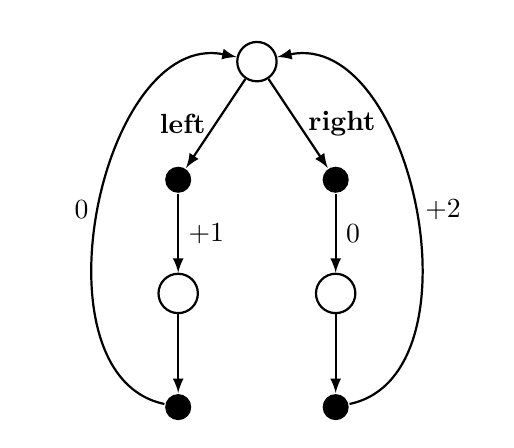
\begin{tikzpicture}[
>=latex, thick ,bend angle=90,
state-node/.style = {circle,thick,draw=black,minimum size=5mm},
action-node/.style = {circle,fill=black, radius=2.5mm, minimum size=2.5mm}
]
   
\node [state-node] (root) at (0, 0) {};
\node [action-node] (l) at (-1, -1.5) {};
\node [action-node] (r) at (1, -1.5) {};

\node [state-node, below=1cm of l] (lmstate) {};
\node [state-node, below=1cm of r] (rmstate) {};

\node [action-node, below=1cm of lmstate] (lm) {};
\node [action-node, below=1cm of rmstate] (rm) {};


% arrows
\draw[->] (root) -- node[midway, left]{\textbf{left}} (l);
\draw[->] (root) -- node[midway, right]{\textbf{right}} (r);
\draw[->] (l) -- node[midway, right]{$+1$} (lmstate);
\draw[->] (r) -- node[midway, right]{$0$} (rmstate);
\draw[->] (lmstate) -- node[midway, left]{} (lm);
\draw[->] (rmstate) -- node[midway, right]{} (rm);

\draw[->] (lm) edge [bend left] node[midway, left]{$0$} (root);
\draw[->] (rm) edge [bend right] node[midway, right]{$+2$} (root);


\end{tikzpicture}
\caption{MDP transition graph}
\label{mdp_transition_graph}
\end{figure}

We can first recall the discounted continuing formulation of the return
\begin{equation}
G_t \doteq \sum_{k=0}^\infty \gamma^k R_{t + k + 1}
\end{equation}

To find what policy is optimal, we need to recall that a policy is better than another one if the value of all states are better, $\pi \geq \pi' \iff v_\pi(s) \geq v_{\pi'}(s),\,  \forall s \in \mathcal{S}$.

\begin{equation}
\begin{split}
v_\pi(\textrm{top state}) &\doteq \mathbb{E}_\pi[G_t \lvert S_t=\textrm{top state}] \\
&= \sum_{a} \pi(a \lvert \textrm{top state}) \sum_{s', r} p(s', r \lvert \textrm{top state}, a) [r + \gamma v_\pi(s')]\\
&= \sum_{s', r} p(s', r \lvert \textrm{top state}, a) [r + \gamma v_\pi(s')],\, a \textrm{ such that } \pi(a | \textrm{top state}) = 1\\
&= \textbf{1}_{\pi = \pi_\textrm{left}} + \gamma \left[2 \cdot \textbf{1}_{\pi = \pi_\textrm{right}} + \gamma v_\pi(\textrm{top state})\right]
\end{split}
\end{equation}

The third equality is due to the deterministic policies and the fourth equality is due to the deterministic transitions after taking an action---taking an action gives always the same reward and always moves the agent into the same state.

The value of the top state can be also written as $\sum_{k=0}^\infty (\gamma^2)^k = \frac{1}{1-\gamma^2}$ if $\pi = \pi_\textrm{left}$ or as $2 \sum_{k=0}^\infty \gamma^{2k + 1} = 2 \gamma \sum_{k=0}^\infty \gamma^{2k} = \frac{2 \gamma}{1-\gamma^2}$ if $\pi = \pi_\textrm{right}$. The equation obtained previously from the Bellman equation gives the same values under their policies.

We can now compute the values of the top state for different $\gamma$; for $\gamma=0$, the agent only looks at the expected immediate reward and $v_{\pi_\textrm{left}}(\textrm{top state}) = 1 > v_{\pi_\textrm{right}}(\textrm{top state}) = 0$. For $\gamma=0.9$, the agent is more farsighted and $v_{\pi_\textrm{left}}(\textrm{top state}) = 5.26 < v_{\pi_\textrm{right}}(\textrm{top state}) = 9.47$ and finally for $\gamma=0.5$, their values are exactly the same.

Let's denote the state in which the agent end up after taking action \textbf{left} as the \textit{left state} and let's also denote the state in which the agent end up after taking action \textbf{right} as the \textit{right state}. The values of the remaining states under $\pi_\textrm{left}$ or $\pi_\textrm{right}$ are

\begin{equation}
\begin{split}
v_{\pi_\textrm{left}}(\textrm{left state}) &= \sum_{k=0}^\infty \gamma^{2k + 1} = \frac{\gamma}{1-\gamma^2}\\
v_{\pi_\textrm{right}}(\textrm{left state}) &= 0 + 2\sum_{k=1}^\infty \gamma^{2k}\\
& = 2\sum_{k=0}^\infty \gamma^{2k} - 1 = 2\frac{1 - (1-\gamma^2)}{1-\gamma^2} = \frac{2 \gamma^2}{1-\gamma^2}\\
\end{split}
\end{equation}


\begin{equation}
\begin{split}
v_{\pi_\textrm{left}}(\textrm{right state}) &= 2 + \sum_{k=0}^\infty \gamma^{2k + 1}\\
& = 2 + \frac{\gamma}{1 - \gamma^2}\\
v_{\pi_\textrm{right}}(\textrm{right state}) &= 2\sum_{k=0}^\infty \gamma^{2k} = \frac{2}{1-\gamma^2}\\
\end{split}
\end{equation}

We have that for $\gamma = 0$, $v_{\pi_\textrm{left}}(\textrm{left state}) = v_{\pi_\textrm{right}}(\textrm{left state})= 0$ and $v_{\pi_\textrm{left}}(\textrm{right state}) = v_{\pi_\textrm{right}}(\textrm{right state})= 2$ because the agent only looks at the immediate rewards and from what we computed previously for the top state, the optimal policy for $\gamma=0$ is $\pi_\textrm{left}$.

For $\gamma = 0.9$, $v_{\pi_\textrm{left}}(\textrm{left state}) = 4.74 < v_{\pi_\textrm{right}}(\textrm{left state})= 8.53$ and

$v_{\pi_\textrm{left}}(\textrm{right state}) = 2 + 4.74 = 6.74 < v_{\pi_\textrm{right}}(\textrm{right state})= 10.53$ because the agent is more farsighted and from what we computed previously for the top state, the optimal policy for $\gamma=0.9$ is $\pi_\textrm{right}$.

For $\gamma = 0.5$, $v_{\pi_\textrm{left}}(\textrm{left state}) = v_{\pi_\textrm{right}}(\textrm{left state})= 2/3$ and

$v_{\pi_\textrm{left}}(\textrm{right state}) = v_{\pi_\textrm{right}}(\textrm{right state})= 8/3$ and from what we computed previously for the top state, for $\gamma=0.5$,  $\pi_\textrm{right}$ and $\pi_\textrm{left}$ are optimal policies.


\paragraph{\textit{Exercise 3.23} (p. 67)} Give the Bellman equation for $q_*$ for the recycling robot.

\bigskip
The Bellman equation for $q_*$ is in general of this form:

\begin{equation}
q_*(s, a) = \sum_{s', r} p(s', r \lvert s, a) \left[r + \gamma \max_{a'} q_*(s', a')\right]
\end{equation}

We will use an equivalent equation based on the three argument function $p$ and three argument function $r$ so we recall the definition of $r(s, a, s')$ that is the expected reward for state--action--next-state triples (($3.6$) in the book at page $49$)
\begin{equation}
\begin{split}
r(s, a, s') \doteq \mathbb{E}[R_{t+1} \lvert S_t = s, A_t = a, S_{t+1} = s'] &= \sum_{r \in \mathcal{R}} r \cdot p(r \lvert s, a, s')\\
&= \sum_{r \in \mathcal{R}} r \cdot \frac{p(s', r \lvert s, a)}{p(s' \lvert s, a)}
\end{split}
\end{equation}

And this gives us $\sum_{s'} p(s' \lvert s, a) \cdot r(s, a, s') = \sum_{s', r} r \cdot p(s', r \lvert s, a)$ and we substitute it in the Bellman equation for $q_*$.

\begin{equation}
\begin{split}
q_*(s, a) &= \sum_{s', r} p(s', r \lvert s, a) \left[r + \gamma \max_{a'} q_*(s', a')\right]\\
&= \left[\sum_{s'} p(s' \lvert s, a) r(s, a, s')\right] + \left[\gamma \sum_{s', r} p(s', r \lvert s, a) \max_{a'} q_*(s', a')\right]\\
&= \sum_{s'} p(s' \lvert s, a) \left[r(s, a, s') + \gamma \max_{a'} q_*(s', a')\right]\\
\end{split}
\end{equation}

Now that we have the equation we want, the Bellman equation for $q_*$ for the recycling robot can be described by a system of these five following non linear equations, one for each state-action pair.

\begin{equation}
\begin{split}
q_*(\textrm{\textbf{h}}, \textrm{\textbf{s}}) &= p(\textrm{\textbf{h}} \lvert \textrm{\textbf{h}}, \textrm{\textbf{s}}) \left[r(\textrm{\textbf{h}}, \textrm{\textbf{s}}, \textrm{\textbf{h}}) + \gamma \max_{a'} q_*(\textrm{\textbf{h}}, a')\right]\\
& + p(\textrm{\textbf{l}} \lvert \textrm{\textbf{h}}, \textrm{\textbf{s}}) \left[r(\textrm{\textbf{h}}, \textrm{\textbf{s}}, \textrm{\textbf{l}}) + \gamma \max_{a'} q_*(\textrm{\textbf{l}}, a')\right]\\
&= \alpha \left[r_\textrm{\textbf{s}} + \gamma \max_{a'} q_*(\textrm{\textbf{h}}, a')\right]\\
& + (1-\alpha) \left[r_\textrm{\textbf{s}} + \gamma \max_{a'} q_*(\textrm{\textbf{l}}, a')\right] \\
&= r_\textrm{\textbf{s}} + \gamma \left[\alpha \max_{a'} q_*(\textrm{\textbf{h}}, a') + (1-\alpha) \max_{a'} q_*(\textrm{\textbf{l}}, a')\right]
\end{split}
\end{equation}

\begin{equation}
\begin{split}
q_*(\textrm{\textbf{h}}, \textrm{\textbf{w}}) &= p(\textrm{\textbf{h}} \lvert \textrm{\textbf{h}}, \textrm{\textbf{w}}) \left[r(\textrm{\textbf{h}}, \textrm{\textbf{w}}, \textrm{\textbf{h}}) + \gamma \max_{a'} q_*(\textrm{\textbf{h}}, a')\right]\\
& + p(\textrm{\textbf{l}} \lvert \textrm{\textbf{h}}, \textrm{\textbf{w}}) \left[r(\textrm{\textbf{h}}, \textrm{\textbf{w}}, \textrm{\textbf{l}}) + \gamma \max_{a'} q_*(\textrm{\textbf{l}}, a')\right]\\
&= 1 \left[r_\textrm{\textbf{w}} + \gamma \max_{a'} q_*(\textrm{\textbf{h}}, a')\right]\\
& + 0 \left[r_\textrm{\textbf{w}} + \gamma \max_{a'} q_*(\textrm{\textbf{l}}, a')\right] =  r_\textrm{\textbf{w}} + \gamma \max_{a'} q_*(\textrm{\textbf{h}}, a')
\end{split}
\end{equation}


\begin{equation}
\begin{split}
q_*(\textrm{\textbf{l}}, \textrm{\textbf{s}}) &= p(\textrm{\textbf{h}} \lvert \textrm{\textbf{l}}, \textrm{\textbf{s}}) \left[r(\textrm{\textbf{l}}, \textrm{\textbf{s}}, \textrm{\textbf{h}}) + \gamma \max_{a'} q_*(\textrm{\textbf{h}}, a')\right]\\
& + p(\textrm{\textbf{l}} \lvert \textrm{\textbf{l}}, \textrm{\textbf{s}}) \left[r(\textrm{\textbf{l}}, \textrm{\textbf{s}}, \textrm{\textbf{l}}) + \gamma \max_{a'} q_*(\textrm{\textbf{l}}, a')\right]\\
&= (1-\beta) \left[-3 + \gamma \max_{a'} q_*(\textrm{\textbf{h}}, a')\right]\\
& + \beta \left[r_\textrm{\textbf{s}} + \gamma \max_{a'} q_*(\textrm{\textbf{l}}, a')\right]\\
&= \beta r_\textrm{\textbf{s}} - 3 (1-\beta) + \gamma \left[(1-\beta) \max_{a'} q_*(\textrm{\textbf{h}}, a') + \beta \max_{a'} q_*(\textrm{\textbf{l}}, a')\right]
\end{split}
\end{equation}


\begin{equation}
\begin{split}
q_*(\textrm{\textbf{l}}, \textrm{\textbf{w}}) &= p(\textrm{\textbf{h}} \lvert \textrm{\textbf{l}}, \textrm{\textbf{w}}) \left[r(\textrm{\textbf{l}}, \textrm{\textbf{w}}, \textrm{\textbf{h}}) + \gamma \max_{a'} q_*(\textrm{\textbf{h}}, a')\right]\\
& + p(\textrm{\textbf{l}} \lvert \textrm{\textbf{l}}, \textrm{\textbf{w}}) \left[r(\textrm{\textbf{l}}, \textrm{\textbf{w}}, \textrm{\textbf{l}}) + \gamma \max_{a'} q_*(\textrm{\textbf{l}}, a')\right]\\
&= 0 \left[r_\textrm{\textbf{w}} + \gamma \max_{a'} q_*(\textrm{\textbf{h}}, a')\right]\\
& + 1 \left[r_\textrm{\textbf{w}} + \gamma \max_{a'} q_*(\textrm{\textbf{l}}, a')\right] =  r_\textrm{\textbf{w}} + \gamma \max_{a'} q_*(\textrm{\textbf{l}}, a')
\end{split}
\end{equation}

\begin{equation}
\begin{split}
q_*(\textrm{\textbf{l}}, \textrm{\textbf{re}}) &= p(\textrm{\textbf{h}} \lvert \textrm{\textbf{l}}, \textrm{\textbf{re}}) \left[r(\textrm{\textbf{l}}, \textrm{\textbf{re}}, \textrm{\textbf{h}}) + \gamma \max_{a'} q_*(\textrm{\textbf{h}}, a')\right]\\
& + p(\textrm{\textbf{l}} \lvert \textrm{\textbf{l}}, \textrm{\textbf{re}}) \left[r(\textrm{\textbf{l}}, \textrm{\textbf{re}}, \textrm{\textbf{l}}) + \gamma \max_{a'} q_*(\textrm{\textbf{l}}, a')\right]\\
&= 1 \cdot \gamma \max_{a'} q_*(\textrm{\textbf{h}}, a')\\
& + 0 \cdot \gamma \max_{a'} q_*(\textrm{\textbf{l}}, a') =  \gamma \max_{a'} q_*(\textrm{\textbf{h}}, a')
\end{split}
\end{equation}

In summary, we have this system of non linear equations:

\begin{equation}
\begin{split}
q_*(\textrm{\textbf{h}}, \textrm{\textbf{s}}) &= r_\textrm{\textbf{s}} + \gamma \left[\alpha \max_{a'} q_*(\textrm{\textbf{h}}, a') + (1-\alpha) \max_{a'} q_*(\textrm{\textbf{l}}, a')\right]\\
q_*(\textrm{\textbf{h}}, \textrm{\textbf{w}}) &=  r_\textrm{\textbf{w}} + \gamma \max_{a'} q_*(\textrm{\textbf{h}}, a')\\
q_*(\textrm{\textbf{l}}, \textrm{\textbf{s}}) &= \beta r_\textrm{\textbf{s}} - 3 (1-\beta) + \gamma \left[(1-\beta) \max_{a'} q_*(\textrm{\textbf{h}}, a') + \beta \max_{a'} q_*(\textrm{\textbf{l}}, a')\right]\\
q_*(\textrm{\textbf{l}}, \textrm{\textbf{w}}) &=  r_\textrm{\textbf{w}} + \gamma \max_{a'} q_*(\textrm{\textbf{l}}, a')\\
q_*(\textrm{\textbf{l}}, \textrm{\textbf{re}}) &= \gamma \max_{a'} q_*(\textrm{\textbf{h}}, a')
\end{split}
\end{equation}


\paragraph{\textit{Exercise 3.24} (p. 67)} Figure $3.5$ (Gridworld) gives the optimal value of the best state of the gridworld as $24.4$, to one decimal place. Use your knowledge of the optimal policy and ($3.8$) to express this value symbolically, and then to compute it to three decimal places.

\bigskip
By using our knowledge of the optimal policy, the dynamics of the environment and how the return is expressed in the discounted continuing case, we can obtain $10 + \gamma v_*(\textrm{\textbf{A'}})$ directly where \textbf{A'} is the state that we end up in after taking any action from \textbf{A}. The expected return from the state \textbf{A} by following the optimal policy is always an immediate reward of $+10$ plus the discounted expected return for the state \textbf{A'} under the optimal policy.

\bigskip
A bit more formally by using the Bellman Optimality equation, the optimal value of state \textbf{A} is
\begin{equation}
\begin{split}
v_*(\textrm{\textbf{A}}) &= \max_{a} \sum_{s', r} p(s', r \lvert \textrm{\textbf{A}}, a) [r + \gamma v_*(s')]\\
&= \sum_{r} p(r \lvert \textrm{\textbf{A}}, a) [r + \gamma v_*(\textrm{\textbf{A'}})]\\
&= r_\textrm{\textbf{A}} + \gamma v_*(\textrm{\textbf{A'}}),\quad r_\textrm{\textbf{A}} = +10
\end{split}
\end{equation}

The second equality comes from the fact that the future next state is the same for all actions in the state \textbf{A}.

\begin{equation}
\begin{split}
v_*(\textrm{\textbf{A}}) &= 10 + 0.9 \cdot 16 = 10 + 9 + 5.4 = 24.400
\end{split}
\end{equation}


\paragraph{\textit{Exercise 3.25} (p. 67)} Give an equation for $v_*$ in terms of $q_*$.

\bigskip
From page $63$ of the book, "Intuitively, the Bellman optimality equation expresses the
fact that the value of a state under an optimal policy must equal the expected return for
the best action from that state"

\begin{equation}
v_*(s) = \sum_{a} \pi(a \lvert s) q_*(s, a) = \max_{a} q_*(s, a)
\end{equation}

where $a \in \mathcal{A}(s)$

\paragraph{\textit{Exercise 3.26} (p. 67)} Give an equation for $q_*$ in terms of $v_*$ and the four-argument $p$.

\bigskip
\begin{equation}
q_*(s, a) = \sum_{s', r} p(s', r \lvert s, a) \left[r + \gamma v_*(s')\right]
\end{equation}

\paragraph{\textit{Exercise 3.27} (p. 67)} Give an equation for $\pi_*$ in terms of $q_*$.

\bigskip

From page $68$ of the book, "Any policy that is greedy with respect to the optimal value functions must be an optimal
policy." and from page $65$, "With $q_*$ the agent does not
even have to do a one-step-ahead search: for any state $s$, it can simply find any action
that maximizes $q_*(s, a)$", translating it into a formula gives us one possible optimal value function:

\begin{equation}
\pi_*(a \lvert s) = \begin{cases} 1 & \textrm{if } a = \argmax\limits_{a'} q_*(s, a')\\ 0 & \textrm{else}\end{cases}
\end{equation}

if we suppose that the argmax gives one of the maximizing actions if many actions achieve the maximum.

\paragraph{\textit{Exercise 3.28} (p. 67)} Give an equation for $\pi_*$ in terms of $v_*$ and the four-argument $p$.

\bigskip
By using the previous exercise and Exercise $3.26$ where
\begin{equation}
q_*(s, a') = \sum_{s', r} p(s', r \lvert s, a') \left[r + \gamma v_*(s')\right]
\end{equation}

we get

\begin{equation}
\pi_*(a \lvert s) = \begin{cases} 1 & \textrm{if } a = \argmax\limits_{a'} \sum_{s', r} p(s', r \lvert s, a') \left[r + \gamma v_*(s')\right] \\ 0 & \textrm{else}\end{cases}
\end{equation}

\paragraph{\textit{Exercise 3.29} (p. 67)} Rewrite the four Bellman equations for the four value functions ($v_\pi$, $v_*$, $q_\pi$,
and $q_*$) in terms of the three argument function $p$ ($3.4$) and the two-argument function $r$
($3.5$).

\bigskip
Let's just first recall how to obtain the three argument function $p$ and the two-argument function $r$ from the $4$ argument function $p$ describing the MDP dynamics:

\begin{equation}
p(s' \lvert s, a) \doteq \sum_{r \in \mathcal{R}} p(s', r \lvert s, a)
\end{equation}

\begin{equation}
r(s, a) \doteq \mathbb{E}[R_{t+1} \lvert S_t = s, A_t= a] = \sum_{r \in \mathcal{R}} r \cdot p(r \lvert s, a) = \sum_{r \in \mathcal{R}} r \sum_{s' \in \mathcal{S}} p(s', r \lvert s, a)
\end{equation}

We can also recall the $4$ Bellman equations for the four value functions:
\begin{equation}
v_\pi(s) = \sum_{a} \pi(a \lvert s) \sum_{s', r} p(s', r \lvert s, a) \left[r + \gamma v_\pi(s')\right]
\end{equation}

\begin{equation}
v_*(s) = \max_{a} \sum_{s', r} p(s', r \lvert s, a) \left[r + \gamma v_*(s')\right]
\end{equation}

\begin{equation}
q_\pi(s, a) = \sum_{s', r} p(s', r \lvert s, a) \left[r + \gamma \sum_{a'} \pi(a' \lvert s') q_\pi(s', a')\right]
\end{equation}

\begin{equation}
q_*(s, a) = \sum_{s', r} p(s', r \lvert s, a) \left[r + \gamma \max_{a'} q_*(s', a')\right]
\end{equation}


where $a \in \mathcal{A}(s)$, $s'$ and $s \in \mathcal{S}$ and $r \in \mathcal{R}$. By replacing all the $4$ Bellman equations with ($3.4$) and ($3.5$) from the book:

\begin{equation}
v_\pi(s) = \sum_{a} \pi(a \lvert s) \left[ r(s, a) + \gamma \sum_{s'} p(s' \lvert s, a) v_\pi(s')\right]
\end{equation}

\begin{equation}
v_*(s) = \max_{a} \left\{ r(s, a) + \gamma \sum_{s'} p(s' \lvert s, a) v_*(s') \right\}
\end{equation}


\begin{equation}
q_\pi(s, a) = r(s, a) + \gamma \sum_{s'} p(s' \lvert s, a) \sum_{a'} \pi(a' \lvert s') q_\pi(s', a')
\end{equation}

\begin{equation}
q_*(s, a) = r(s, a) + \gamma \sum_{s'} p(s' \lvert s, a) \max_{a'} q_*(s', a')
\end{equation}

As remark, the Bellman equation with two-argument function $r$ and three-argument  function $p$ could be used directly to obtain the last equality for $v_*(\textrm{\textbf{h}})$ or the equation for $v_*(\textrm{\textbf{l}})$ in Example $3.9$ on the Bellman Optimality Equation for Recycling Robot (p. 65).

\paragraph{Proof of the formula used in the first equality of Example $3.9$ Bellman Optimality Equation for Recycling Robot (p. 65)}

We want to prove that 
\begin{equation}
v_*(s) = \max_{a} \sum_{s'} p(s' \lvert s, a) \left[r(s, a, s') + \gamma v_*(s')\right]
\end{equation}

Recall the definition of $r(s, a, s')$ that is the expected reward for state--action--next-state triples (($3.6$) in the book at page $49$)
\begin{equation}
\begin{split}
r(s, a, s') \doteq \mathbb{E}[R_{t+1} \lvert S_t = s, A_t = a, S_{t+1} = s'] &= \sum_{r \in \mathcal{R}} r \cdot p(r \lvert s, a, s')\\
&= \sum_{r \in \mathcal{R}} r \cdot \frac{p(s', r \lvert s, a)}{p(s' \lvert s, a)}
\end{split}
\end{equation}

And this gives us $\sum_{s'} p(s' \lvert s, a) \cdot r(s, a, s') = \sum_{s', r} r \cdot p(s', r \lvert s, a)$ and we substitute it in the Bellman equation for $v_*$.

\begin{equation}
\begin{split}
v_*(s) &= \max_{a} \sum_{s', r} p(s', r \lvert s, a) \left[r + \gamma v_*(s')\right]\\
&=\max_{a}\left\{\sum_{s'} p(s' \lvert s, a) \cdot r(s, a, s') + \gamma \sum_{s', r} p(s', r \lvert s, a) v_*(s')\right\}\\
&= \max_{a} \sum_{s'} p(s' \lvert s, a) \left[r(s, a, s') + \gamma v_*(s')\right]
\end{split}
\end{equation}

This proves the formula.

\end{document}